% ****** Start of file RamanCoolingV1.tex ******
%
%
% See the REVTeX 4 README file
% It also requires running BibTeX. The commands are as follows:
%
%

\documentclass[%
 reprint,
%superscriptaddress,
%groupedaddress,
%unsortedaddress,
%runinaddress,
%frontmatterverbose, 
%preprint,
%showpacs,preprintnumbers,
%nofootinbib,
%nobibnotes,
%bibnotes,
 amsmath,amssymb,
 aps,
prl,
%pra,
%prb,
%rmp,
%prstab,
%prstper,
%floatfix,
]{revtex4-1}

\usepackage{graphicx}% Include figure files
\usepackage{dcolumn}% Align table columns on decimal point
\usepackage{bm}% bold math
%\usepackage{hyperref}% add hypertext capabilities
%\usepackage[mathlines]{lineno}% Enable numbering of text and display math
%\linenumbers\relax % Commence numbering lines

%\usepackage[showframe,%Uncomment any one of the following lines to test 
%%scale=0.7, marginratio={1:1, 2:3}, ignoreall,% default settings
%%text={7in,10in},centering,
%%margin=1.5in,
%%total={6.5in,8.75in}, top=1.2in, left=0.9in, includefoot,
%%height=10in,a5paper,hmargin={3cm,0.8in},
%]{geometry}

\begin{document}

%\preprint{APS/123-QED}

\title{A Plugged Trap for Crossed Field Spin-Flip Loss}%


\author{David Reens}%
\author{Hao Wu}
\author{Tim Langen}%
\author{Jun Ye}
\affiliation{%
 Physics Department, University of Colorado at Boulder\\
}%

\date{\today}% It is always \today, today,


%%%%%%%%%%%%%%%%%%%%%
%ABSTRACT
%%%%%%%%%%%%%%%%%%%%%
\begin{abstract}
A new electromagnetic trap geometry allows tunable plugging of non-adiabatic spin flip loss in crossed electric and magnetic fields. This loss afflicts a wide set of candidate molecules and operates at much higher temperatures compared with the more familiar atomic spin-flip loss near the zero of a magnetic trap, and thus it's removal represents an important step toward ultracold molecules. Using only an external magnetic bias coil, the loss rate is tuned from over $100 \text{ s}^{-1} $ to below the vacuum limited lifetime in a $100 \text{ mK}$ sample of OH molecules.
\end{abstract}


\maketitle


%%%%%%%%%%%%%%%%%%%%%%%%%%%%%%%%%
%
%     III   NNN   TTT   RRR   OOO   DDD   UUU   CCC   TTT   III   OOO   NNN
%     III   NNN   TTT   RRR   OOO   DDD   UUU   CCC   TTT   III   OOO   NNN
%     III   NNN   TTT   RRR   OOO   DDD   UUU   CCC   TTT   III   OOO   NNN
%
%%%%%%%%%%%%%%%%%%%%%%%%%%%%%%%%%
%\section{Introduction}
The ultracold regime extends toward molecules on many fronts. Several bialkali molecules are available and others are under development. Creative and carefully engineered laser cooling strategies are tackling certain nearly rotationally diagonal molecules. A plethora of non-optical cooling strategies have succeeded to greater or lesser extents on other molecules. All of these molecules will require secondary strategies like evaporation or sympathetic cooling to make further gains in phase space density. They also may face a familiar challenge: spin flip loss near the zero of a magnetic trap, only dramatically enhancemed for certain molecules. Here we report on our encounter with OH molecule enhanced spin flip loss and our solution.

The knowledge of spin flips or Majorana hops as an eventual trap lifetime limit predates the very first magnetic trapping of neutrals\cite{Migdall1985}. Spin flips were directly observed and overcome in the TOP trap\cite{Petrich1995}, and shortly later with a plugged dipole trap\cite{Davis1995}, famously enabling the first Bose-Einstein condensates. The molecular spin-flips can occur at much higher temperatures compared with their atomic counterpart, and thus they need to be addressed much earlier than might have been expected. The magnitude of the loss varies with molecular species, and is particularly strong for the case of the neutral hydroxyl radical (OH) that we study, but is nonetheless remarkably general.

We begin with a more thorough explanation of this crossed field spin flip loss mechanism and its applicability to molecular species than is currently to our knowledge available. We then present our electromagnetic trap geometry, which not only overcomes this loss, but does so in a tunable manner, allowing us to fully validate our explanation of the loss with experimental data.


%%%%%%%%%%%%%%%%%%%
%  EXPLAIN THE LOSS MECHANISM
%%%%%%%%%%%%%%%%%%%
%\section{Loss Mechanism  \label{sec:lm} }
Successful magnetic trapping is predicated on an adiabatic criterion: the internal spin of the trapped species must follow the changes in direction of the external field. Equivalently, rotation of the external field constitutes a coupling between the two or more internal spin states of the species with respect to the field. The energetic separation of the states must dwarf this coupling or spin-flips will occur. Consider a spin $1/2$ atom traveling at velocity $v$ parallel to the strong axis of a quadrupole trap $\vec{B}=B'z\hat{z}-B'x\hat{x}/2-B'y\hat{y}/2$. The atom is offset from the axis by a distance $2a$ in the $x$ direction, so that from its perspective, $\vec{B}(t)=B'vt\hat{z} + B'a\hat{x}$. Working in the familiar basis of Pauli spin matrices, the Hamiltonian for this atom is thus

\begin{equation}
H(t) = \frac{1}{2}\mu_BB'(2vt\boldsymbol{\sigma_z} + a\boldsymbol{\sigma_x}) = \begin{pmatrix} \alpha t & \beta \\ \beta & -\alpha t \end{pmatrix}
\end{equation}

\noindent Where terms are gathered as $\alpha$ and $\beta$ for clarity. Beginning at $t=-\infty$ in the higher energy state, the Landau-Zener formula gives the chances of hopping to the lower energy untrapped state by the time $t=\infty$:

\begin{equation}
P_{\text{diabatic}}=e^{-\pi\beta^2 /(\hbar\alpha)}
\end{equation}

\noindent Usually we think of couplings like $\beta$ as increasing the possibility of state transfer, but note that in this basis, when $t$ crosses through zero the ``trapped" state or the state with higher energy changes from the bottom right to the top left of the Hamiltonian. So while $\beta$ does lead to transfer, in this case ``transfer" is equivalent to remaining trapped. Larger $\beta$ actually reduces the rotation rate of the magnetic field which couples trapped and untrapped states.

%\subsection{Molecules}
\begin{figure}[b]
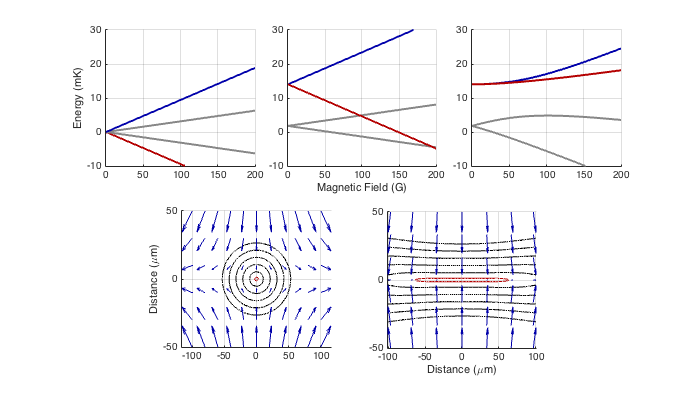
\includegraphics[width=70mm]{blocking.png}%
\caption{
The blocking effect. (a), four Zeeman split lines in the ground state of OH. A nearly identical set of four states of opposite parity lie 100 mK below. The trapped state and it's spin flip partner are in blue and red. (b) Zeeman splitting with the addition of an electric field of 150 V/cm parallel to the magnetic field. (c) Again but with the fields orthogonal. (d) Contours showing the gap between blue and red states near the zero of a magnetic quadrupole trap without electric field. (e) Again with 150 V/cm. Note the drastic widening of the lowest contour, but without significant reduction in slope approaching it.
\label{fig:blocking}}
\end{figure}

Now we add a homogeneous electric field in the z-direction. For Hund's case (a) molecules, the Stark and Zeeman perturbations are not mutually diagonal\cite{Lara2008}, and thus the effects combine differently depending on the angle between the fields. For OH molecules in their $^2\Pi_{3/2}$ ground state moving parallel to the strong axis as before, the Hamiltonian becomes: 

\begin{equation}
aoeu
\end{equation}

With parallel fields the effects are purely additive, but with perpendicular fields they are less so. In fact, the presence of one field can be thought of as ``blocking" the effect of the second field. In Fig.~\ref{fig:blocking}, the Zeeman effect in the presence of an orthogonal electric field is compared to that with a parallel field of the same magnitude and without any electric field. It is seen that the electric field blocks the Zeeman effect from linear to quadratic for ground state $^2\Pi_{3/2}$ weak field seeking OH, and that the energy separation between the top two states is further blocked to cubic in magnetic field:

\begin{equation}
\label{eq:HZprop}
H_Z\propto \frac{B^3}{E^4}f(\Delta,E)\Delta
\end{equation}

\noindent Here $B$, $E$, and $\Delta$ are Zeeman, Stark, and lambda doublet energies with all coefficients subsumed. $f$ is a function of lambda doublet and stark energy with units of energy that approaches $\Delta$ for $E << \Delta$ but $E$ for large $E$. This blocking means that when the conditions $B<<E$ and $B\cdot E=0$ are met, the energy gap between the highest two states will be much smaller than what one would expect from the magnetic energy alone. Near the zero of a magnetic quadrupole with homogeneous electric field applied, both conditions are met along a plane through the origin thanks to the rotation of the magnetic field about the zero. 

Of course, transfer between the highest two states does not necessarily mean immediate loss depending on the character of the second highest state. Where $B<<E$, the second state is opposite in magnetic field dependence, and so one might think elsewhere in the trap where $B>E$ it would be untrapped. However, the electric field also opens various transition zones where a molecule may adiabatically follow into the other magnetic spin states between aligned and antialigned, with the result that this second highest state is mostly trapped, with the exception of a few holes similar to the one between the top two states for $B<<E$ and $B\cdot E = 0$, and with a reduced absolute trap depth related to $\Delta$. 

We can be more precise and develop a scaling law for the enhancement. Let $\kappa$ be the threshold for gaps between states below which spin-flips are possible at the 50\% level. $\kappa$ depends on the velocity of trapped species, but suppose we have a specific temperature of interest, and therefore a mean velocity. Without electric field, the effective cross sectional area for a hopping region is $\pi \kappa^2$, since loss can occur where $B<\kappa$. With electric field, we have from eq.~\ref{HZprop}

\begin{equation}
B < \sqrt[3]{\frac{\kappa E^4}{f(\Delta,E)\Delta}}
\end{equation}

\noindent With $E<<\kappa$ there is no enhancement. (Nor is there any reduction, the Zeeman effect returns to linear by the time $B$ reaches $\kappa$. For $E>\sqrt[4]{\kappa^2\Delta f(\Delta,E)}~\sqrt{\kappa\Delta}$, there is an enhancement. We can assume $E<\Delta$ since $\kappa<<\Delta$ at temperatures of interest. In terms of loss area, the enhancement factor is given by:

\begin{equation}
\nu = \left(\frac{E^4}{\kappa^2\Delta^2}\right)^\frac{2}{3}
\label{eq:blimit}
\end{equation} 

It is interesting to note that in ref.~\cite{Lara2008}, it was specifically undertaken to investigate the spin-flip loss for OH molecules in a magnetic quadrupole trap with superposed electric field, and no enhancement was found. This turns out to be a consequence of a reasonable yet false assumption that a 4-state approximate Hamiltonian with two spin states and two parities would contain the behavior relevant for spin-flip loss in mixed fields. This approximate Hamiltonian exhibits only constant order blocking- i.e. the Zeeman effect remains linear though with adjusted slope. This is intuitively reasonable, because with two spin states, the Zeeman effect has to break the Stark effect's coupling of opposite spin states, a 1st order task, but a 3rd order when there are 4 spin states and the states coupled by the Stark effect are three magnetic quanta apart. More recent work in our lab correctly recognized the importance of the effect and accounted for it, although this was done numerically with no algebraic counterpart.

This effect will influence any case (a) molecule with more than two magnetic states such as NO ($X^2\Pi_{3/2}$), and it will also influence case (b) molecules in accordance with the strength of their non-zero spin-rotation coupling often denoted $\gamma$. (I'd like to check how much this enhances loss for YO and SrF, but I haven't done it yet). It also might crop up with superposed optical and magnetic fields, though I haven't tried to check.

%%%%%%%%%%%%%%%%%%%%%%%%%%
%  PIN TRAP GEOMETRY
%%%%%%%%%%%%%%%%%%%%%%%%%%
\section{Pin Trap Geometry \label{sec:ptg} }
One obvious way to avoid the loss enhancement is to simply never use electric field in a magnetic trap. This prevents loss from being enhanced compared with atoms, but doesn't remove it entirely. Another possibility is to trap with electric fields, where no spin-flip loss is possible thanks to the large lambda-doublet splitting. However this splitting also results in a significant reduction in trap gradient close to the trap center, very undesirable for further cooling by evaporation, which needs as much phase space density as possible.

Another option would be to apply electric fields nowhere orthogonal to magnetic, for example overlapped quadrupole fields. In this case the loss is neither enhanced nor entirely removed, but perfect alignment is required. If the zeros do not overlap, there is a loss region whose size is set by the misalignment. 

Seeking to remove the loss entirely but without any trap gradient sacrifice, we developed a solution that requires devoting both electric and magnetic fields to trapping, but is in all other respects a best-case scenario. Instead of avoiding orthogonal fields entirely, the geometry simply ensures that the magnetic field is not too close to zero when they are orthogonal. The key idea is to use a 2D instead of a 3D magnetic quadrupole, apply a homogeneous bias magnetic field in the untrapped direction to prevent the magnetic field from having any zeros, and trap in the third direction with electric fields. The fields can be approximated as follows:

\begin{eqnarray}
\vec{B} &=&  B^\prime y\hat{x}+ B^\prime x\hat{y} + B_{coil} \hat{z}\\
\vec{E} &=&  E^\prime y\hat{y}-  E^\prime z\hat{z}
\end{eqnarray}

In other words 2D quadrupole traps in the xy plane for B and in the yz plane for E. Now E is perpendicular to B when:
\begin{eqnarray}
\vec{B}\cdot \vec{E} &= 0\\
B^\prime x E^\prime y - B_{coil}  E^\prime z &= 0\\
B_{coil}z &= xyB^\prime
\end{eqnarray}

So we see that E and B are perpendicular on a hyperbolic sheet which deviates more significantly from the z axis with increasing $B_{coil}$, and reduces to the pair of planes $x=0$ and $y=0$ in the limit that $B_{coil} = 0$. On this hyperbolic sheet, B must be larger than the threshold set by Eq.~\ref{eq:blimit}. In fact, the volume everywhere in which the limit is satisfied can be directly solved. 

\begin{equation}
|B|^3 = \left(B'^2(x^2+y^2)+B_{\text{coil}}^2\right)^3 < \begin{cases} \kappa E'^4(y^2+z^2)^2/\Delta^2,  E'\sqrt(y^2+z^2)<\Delta\\ E'^3(y^2+z^2)^{3/2} /\Delta, E'\sqrt(y^2+z^2)>\Delta\end{cases}
\end{equation}

In our experiment, $B' \approx 5 \text{T/cm} \times 1.4\mu_\text{B}$, and $E' ~ 120 \text{kV/cm}^2 \times 1.67 d_E$, so $B'/E' ~ 1$. 

When $B\cdot E = 0$, the B field must be larger than the limit where $\mu_eE >> \mu_b B$, i.e. close to the z-axis since that is where $B$ is small, and further from $z=0$ since that is where $E$ is large. You can see the loss regions plotted as a function of $B_{coil}$, with $B_{pin}$ set to zero in Fig.~\ref{fig:LSurfs}.

Notably, $B_{coil}$ tunes the proximity of the loss regions to the trap center, and is thus potentially useful as a knife for spectroscopy or evaporation.

\begin{figure}[b]
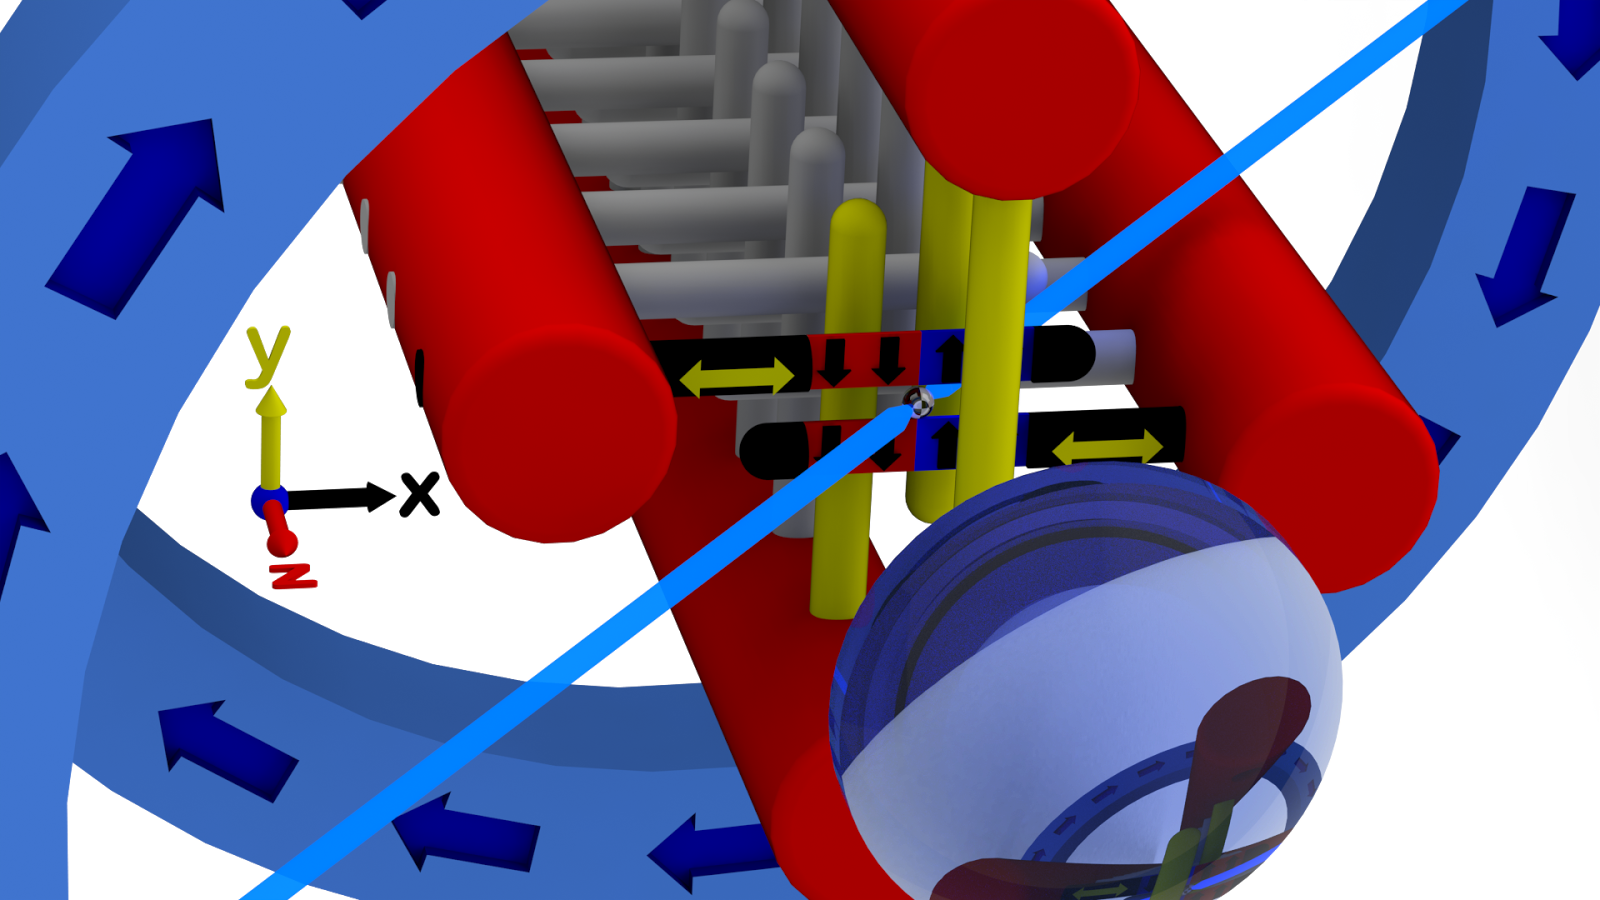
\includegraphics[width=70mm]{blue-red-yellow-v2_CAD.png}%
\caption{
OH molecules are created using a supersonic expansion source and decelerated from an initial velocity of 460m/s to a final velocity of 40ms/s using a Stark decelerator (red). The decelerator contains 142 electrode pairs (gray). Trapping is achieved by combining a radial magnetic quadrupole field, created by the magnetized second to last electrode pair of the decelerator, with a longitudinal electric quadrupole field created by the third to last and last electrode pairs, respectively (yellow, one electrode is omitted for clarity). The magnetized electrodes can be translated in situ along the x-axis to align their domains and optimize the quadrupole. As there is no trapping magnetic field in the z-direction in this configuration, macroscopic external bias coils can be used to lift the gap between the top two states of the OH ground-state manifold and thus tune the molecular loss. Detection is realized using laser induced fluorescence along the x+y-z direction (blue), which is collected using a lens system and PMT in the z-direction.
\label{fig:CAD}}
\end{figure}


\begin{figure}[b]
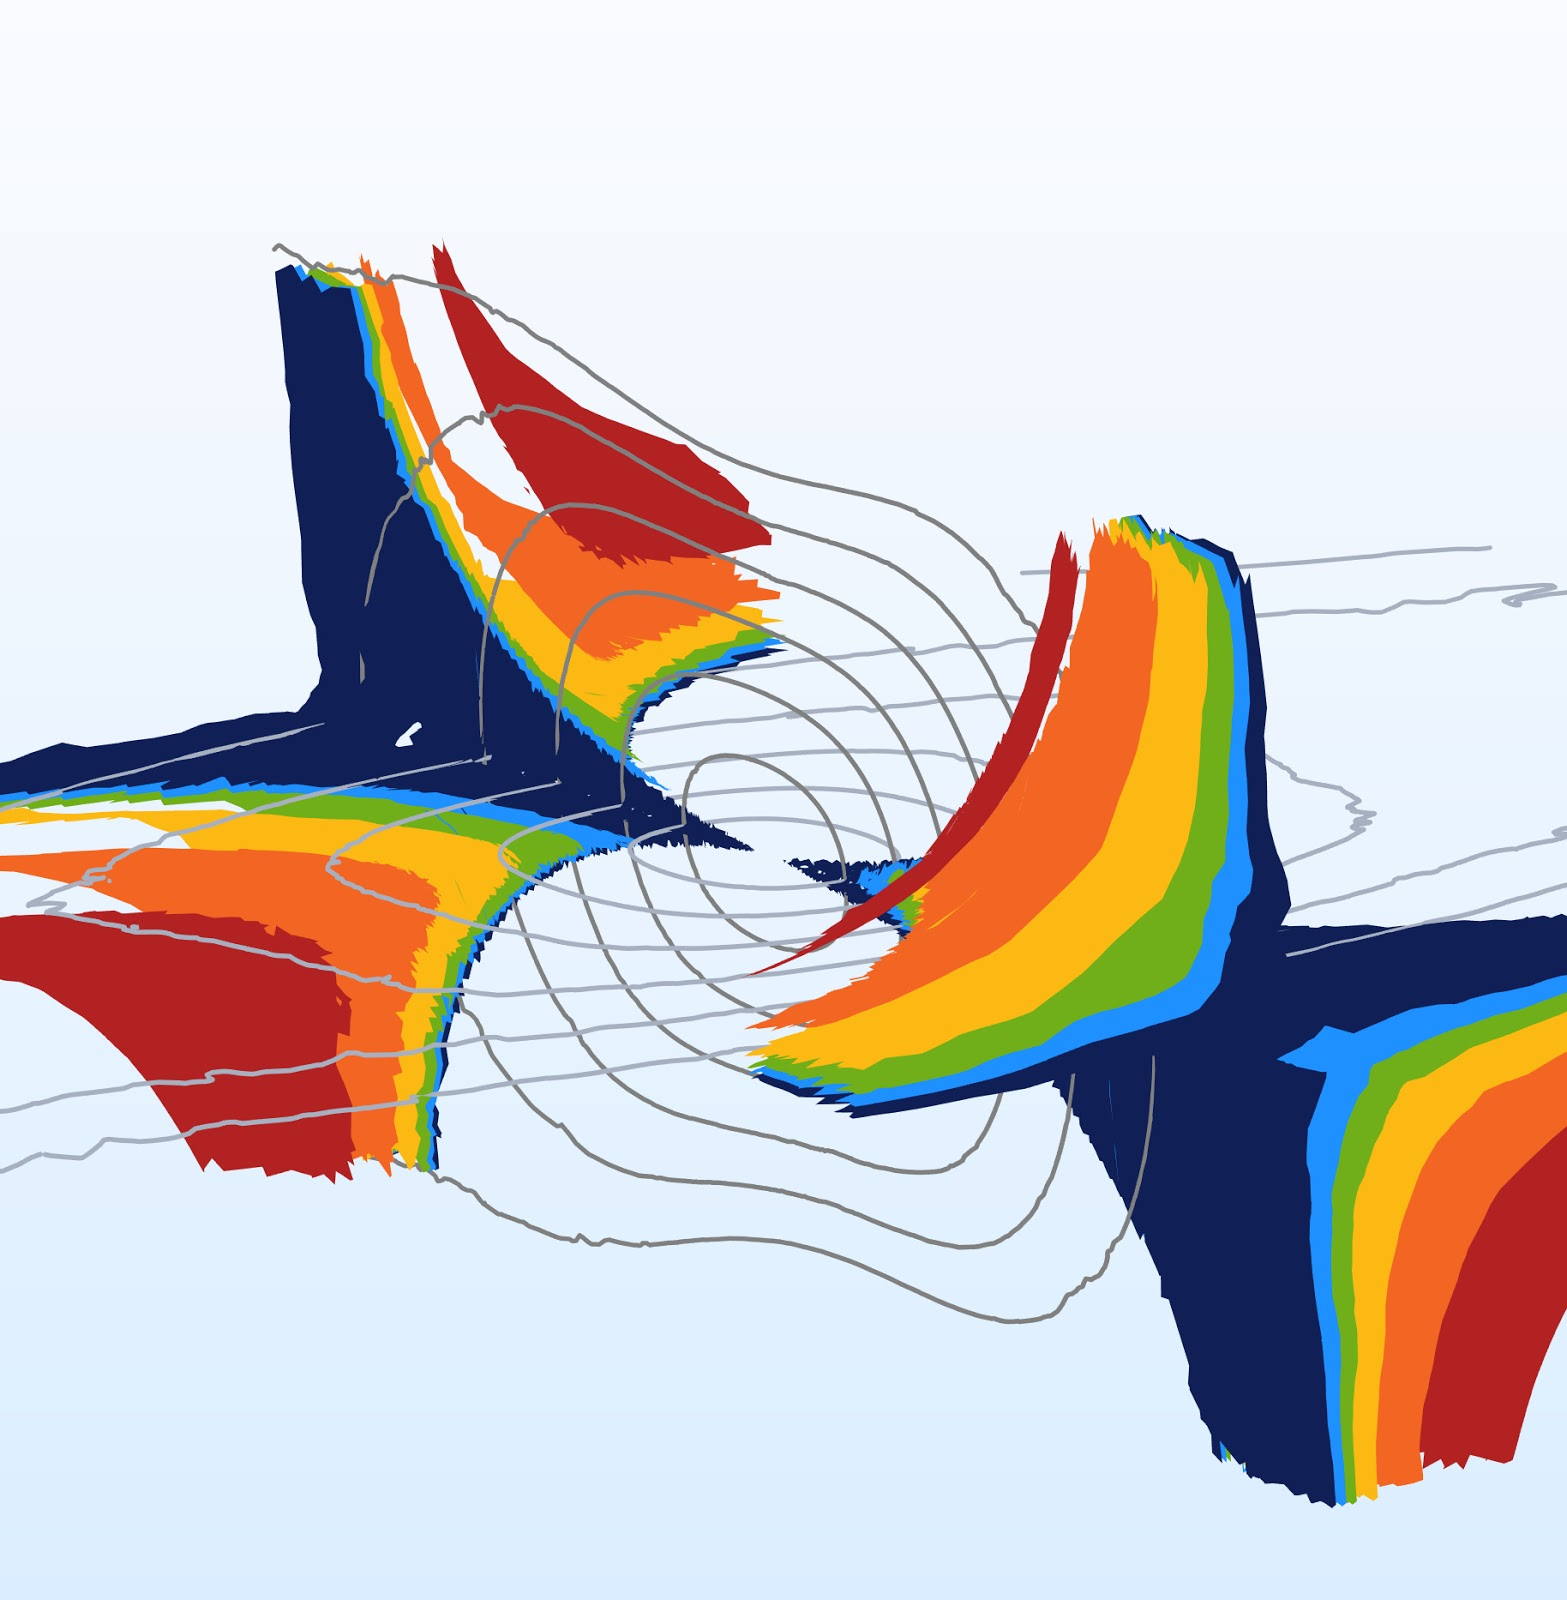
\includegraphics[width=70mm]{Loss_Surface_Chunks_0-320_0.jpeg}%
\caption{
Contours every 100mK, colors 0,20,40,80,160,320 G bias field and pin offset at zero. Molecules can spin-flip and be lost, whenever they cross these areas.
\label{fig:LSurfs}}
\end{figure}

%%%%%%%%%%%%%%%%%%%
%  LOSS TRAJECTORY DATA
%%%%%%%%%%%%%%%%%%%
\section{Loss Trajectories}
We can measure OH population in the trap as a function of time and as a function of bias field used for removing the loss. This demonstrates how truly wonderful and amazing we are.


%includes uncited bib entries
\nocite{*}


\bibliography{MolecularMajoranaLoss.bib}% Produces the bibliography via BibTeX.

\end{document}
%
% ****** End of file MolecularMajoranaLoss.tex ******
